\refstepcounter{figure}
\noindent Figure \thefigure\ shows jitter variation.

\begin{center}
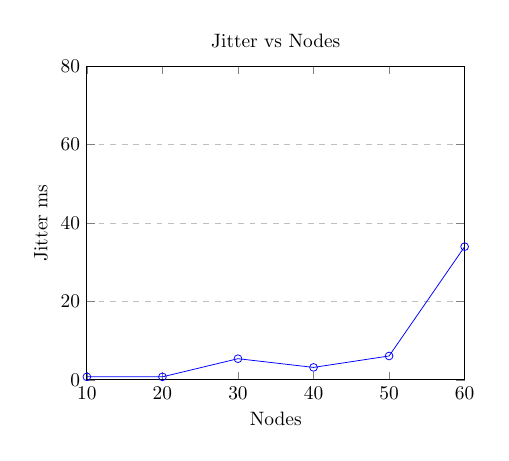
\begin{tikzpicture}[scale=0.7]
\begin{axis}[
title={Jitter vs Nodes},
xlabel={Nodes}, ylabel={Jitter ms},
xmin=10, xmax=60, ymin=0, ymax=80,
xtick={10,20,30,40,50,60},
ymajorgrids=true, grid style=dashed,
]

\addplot[color=blue, mark=o] coordinates {(10,0.77) (20,0.77) (30,5.40) (40,3.18) (50,6.09) (60,33.96)};


\end{axis}
\end{tikzpicture}

\textbf{Figure \thefigure: Jitter vs Nodes}
\label{fig:jitter_density}
\end{center}